\documentclass[tikz,border=8pt]{standalone}
\usepackage{tikz}
\usetikzlibrary{arrows.meta,positioning}

\begin{document}
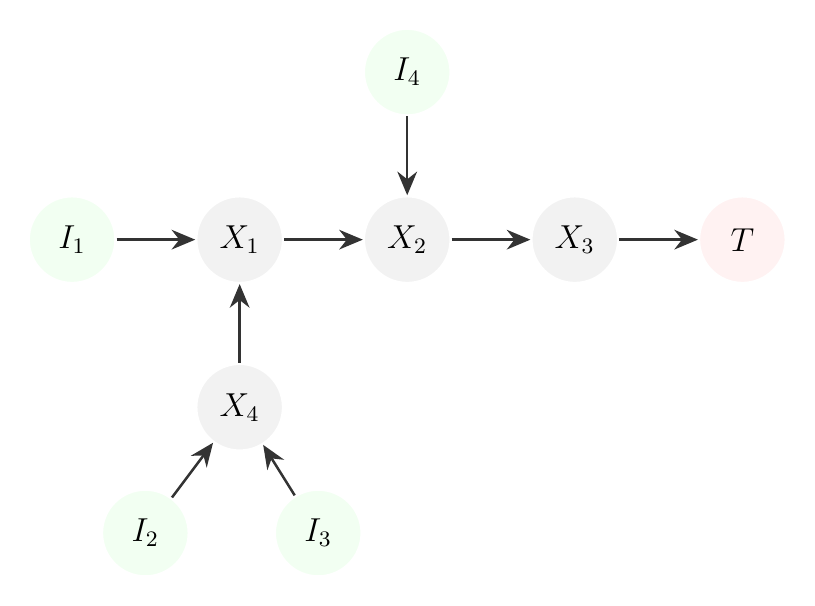
\begin{tikzpicture}[
    >={Stealth[length=3mm,width=2.5mm]},
    node distance=10mm,
    every node/.style={font=\large},
    ing/.style={
        circle, draw=white, line width=0.8pt,
        minimum size=11mm, inner sep=0pt,
        fill=green!5
    },
    tar/.style={
        minimum size=11mm, inner sep=0pt,
        circle, draw=white, line width=0.8pt,
        fill=red!5
    },
    inter/.style={
        circle, draw=white, line width=0.8pt,
        minimum size=11mm, inner sep=0pt,
        fill=gray!10
    },
    arr/.style={->, line width=0.9pt, black!80}
]

    % Main horizontal chain
    \node[ing]   (I1)  {$I_1$};
    \node[inter] (X1) [right=of I1] {$X_1$};
    \node[inter] (X2) [right=of X1] {$X_2$};
    \node[inter] (X3) [right=of X2] {$X_3$};
    \node[tar]   (T)  [right=of X3] {$T$};

    % I4 above X2
    \node[ing] (I4) [above=of X2] {$I_4$};

    % X4 below X1
    \node[inter] (X4) [below=of X1] {$X_4$};

    % I2 and I3 feeding I4 from below
    \node[ing] (I2) [below left=8mm and 4mm of X4]  {$I_2$};
    \node[ing] (I3) [below right=8mm and 2mm of X4] {$I_3$};

    % Edges
    \draw[arr] (I1)  -- (X1);
    \draw[arr] (X1) -- (X2);
    \draw[arr] (X2) -- (X3);
    \draw[arr] (X3) -- (T);
    \draw[arr] (I4)  -- (X2);
    \draw[arr] (X4) -- (X1);
    \draw[arr] (I2)  -- (X4);
    \draw[arr] (I3)  -- (X4);

\end{tikzpicture}
\end{document}
